\documentclass[12pt, a4paper]{article}

\usepackage[T1]{fontenc}
\usepackage{graphicx}
\usepackage{mathptmx}
\usepackage{ragged2e}

\graphicspath{{../img}}

\pagenumbering{gobble}
\date{}

\begin{document}

  \begin{flushleft}

    \textbf{Assignment Week 3}
    \linebreak

    \textbf{Star Role Club: Cybersecurity - Honeypots}
    \linebreak

    \textbf{Oleh: Radinal Shidiq Saragih}

    \textbf{Mentor Muhamad Rifki Arisagas}

  \end{flushleft}

  \section*{Essay}

    Honeypot di dunia Cybersecurity adalah istilah sistem atau aplikasi komputer
    yang digunakan sebagai "jebakan" bagi seorang hacker.

    Honeypot akan bertindak seperti aplikasi atau service seperti biasanya,
    namun semua hal yang dilakukan terhadap aplikasi atau dalam service tersebut
    akan disimpan untuk dianalisis hingga dapat menjadi penilaian terhadap sistem
    keamanan yang ada di sistem produksi ataupun untuk mencari tahu indentitas
    dari yang menyerang.

    Honeypot ini secara konsep sangat mirip dengan virus komputer malware, karena
    keduanya akan "berpura-pura" sebagai hal lain di sistem komputer tersebut.

    Honeypot biasa digunakan oleh penegak hukum untuk menjebak kriminal di dunia
    cyber, khususnya di dark web yang banyak terdapat situ member-only yang memperdagangkan
    hal-hal ilegal, hingga ada percentase tinggi jumlah situs honeypot yang ada disana
    untuk menjebak kriminal-kriminal tersebut.

    Honeypot dalam ranah keamanan sistem pun kerap dimanfaatkan untuk menambah
    inteligensi dan adaptabilitas sistem terhadap serangan-serangan baru, contoh yang
    paling umum adalah untuk menambah keakuratan sistem IDS atau Intrution Detection
    System, yang bertugas untuk menditeksi tindakan-tindakan mencurigakan di suatu
    sistem, sistem ini jika di kolaborasikan dengan Honeypot akan menambah keakuratan dalam
    bagaimana ia menditeksi serangan-serangan yang akan bermunculan.

    Bedasarkan tingkatan atau besarnya interaksi, terdapat tiga jenis, yaitu.

    \begin{itemize}
      \item Pure Honeypot

        Sebuah sistem produksi utuh yang akan mengawasi semua aktifitas hacker
        melalui sebuah Bug-Tap (Listening Device) yang akan menjadi middle-man
        antara sistem tersebut dengan internet.

      \item High-Interaction Honeypot

        Honeypot yang meniru berbagai service di dalam sebuah sistem produksi,
        dan biasanya juga memanfaatkan beberapa sistem virtual agar lebih
        terlihat meyakinkan sebagai sistem internal sebuah perusahaan atau jasa.

        Honeypot yang di tingkatan ini tergolong sulit untuk terditeksi
        sebagai honeypot oleh hacker karena memiliki banyak karakteristik
        seperti sistem sebenarnya.

      \item Low-Interaction Honeypot

        Honeypot di tingkatan ini hanya meniru beberapa service di sistem yang
        secara umumnya akan ditarget oleh seorang hacker, honeypot jenis ini
        memiliki kelebihan dalam penggunaaan resources sistem yang ringan dan
        kemudahan untuk di deploy.

    \end{itemize}

    Dan bedasarkan dengan tujuan dari honeypot tersebut terdapat dua jenis, yaitu.

    \begin{itemize}

      \item Production Honeypots

        Honeypot yang berada di dalam sistem produksi dan digunakan untuk meningkatkan
        kemampuan sistem keamanan untuk menditeksi adanya serangan. Honeypot jenis
        ini biasanya hanya bersifat Low-Interaction honeypot.

      \item Research Honeypots

        Honeypot yang dijalankan dengan tujuan untuk menjadi information-gatherer
        dari taktik atau motif di balik serangan cyber. Research Honeypots jauh lebih
        kompleks secara struktural dibandingkan Production Honeypots karena biasanya
        meniru sebuah sistem utuh atau Pure Honeypot atau setidaknya sebuah
        High-Interaction honeypot.

    \end{itemize}

  \section*{Demonstrasi Honeypot}

  Tujuan dari demonstrasi ini adalah untuk memberikan contoh sederhanan dari
  konsep sebuah honeypot. Jenis honeypot yang digunakan adalah honeyport, yaitu
  honeypot yang dalam skala lebih kecil lagi, honeypot jenis ini biasanya akan
  meniru sebuah port di dalam suatu sistem.

  Honeyport yang akan didemonstrasikan hanya akan mendengarkan ke satu port yang
  opened atau terbuka di sistem, dan secara default akan me-blacklist ip yang
  mencoba menghubung ke port tersebut menggunakan iptables, jadi secara sifat honeypot ini bersifat
  mirip dengan sistem IDS atau Intrusion Detection System namun lebih sederhana.

  \begin{center}
    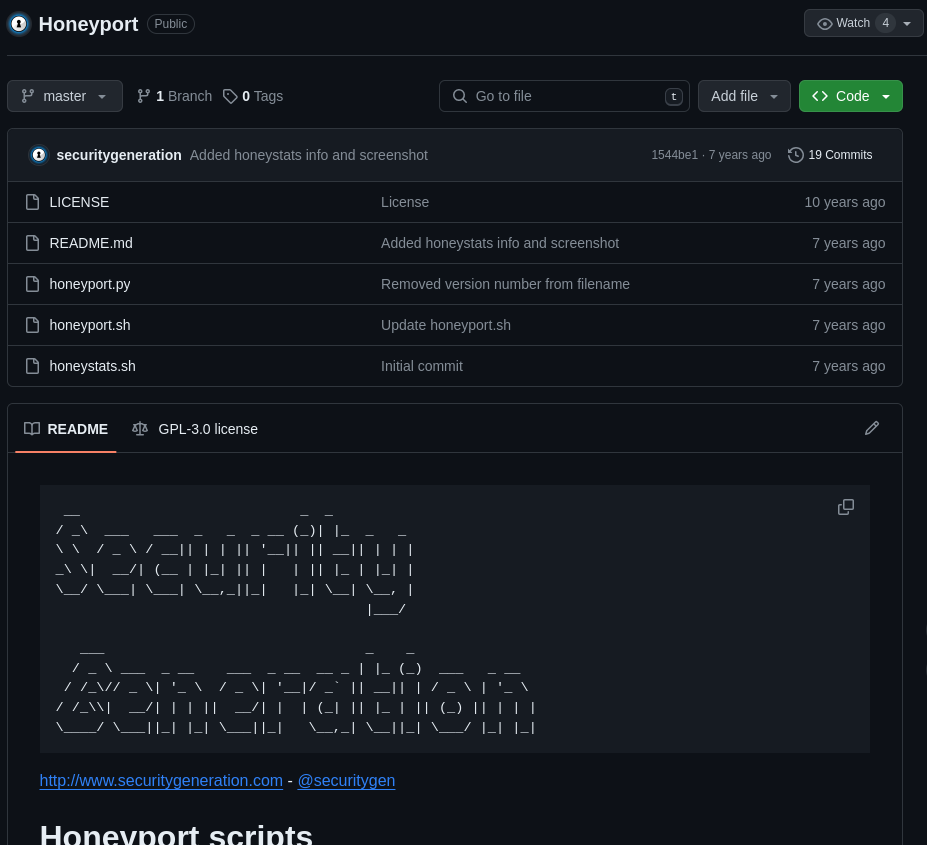
\includegraphics[scale=0.4]{HONEYPORTPAGE}
  \end{center}

  Honeypot yang digunakan bernama "Honeyport" dan source codenya dapat dilihat di github
  (https://github.com/securitygeneration/Honeyport).

  Terdapat dua versi script yang disediakan di repository, satu script python, dan
  satunya lagi script bash atau shell. Kedua script yang tersedia kurang lebih
  serupa, namun script python dikatakan di dokumentasinya memiliki fitur yang
  lebih banyak dan mudah untuk mengintegrasikan dengan module atau plugin-plugin
  honeypot lain.

  Honeyport ini sendiri biasanya digunakan bersamaan dengan honeypot lain yang
  akan memberi tampilan seakan-akan script ini adalah suatu service umum di
  server web.

  Yang akan di demonstrasi kan di kali ini adalah script bashnya, hal ini dikarenakan
  terdapat conflict di versi python yang tersedia di repository debian dengan
  versi python yang didalam script tersebut, hingga tidak memungkinkan untuk dijalankan.

  Environment dimana demonstrasi akan dilakukan adalah di sebuah Virtual Machine
  Debian 11 minimal yang terhubung ke client atau mesin utama saya melalui SSH.

  \begin{center}
    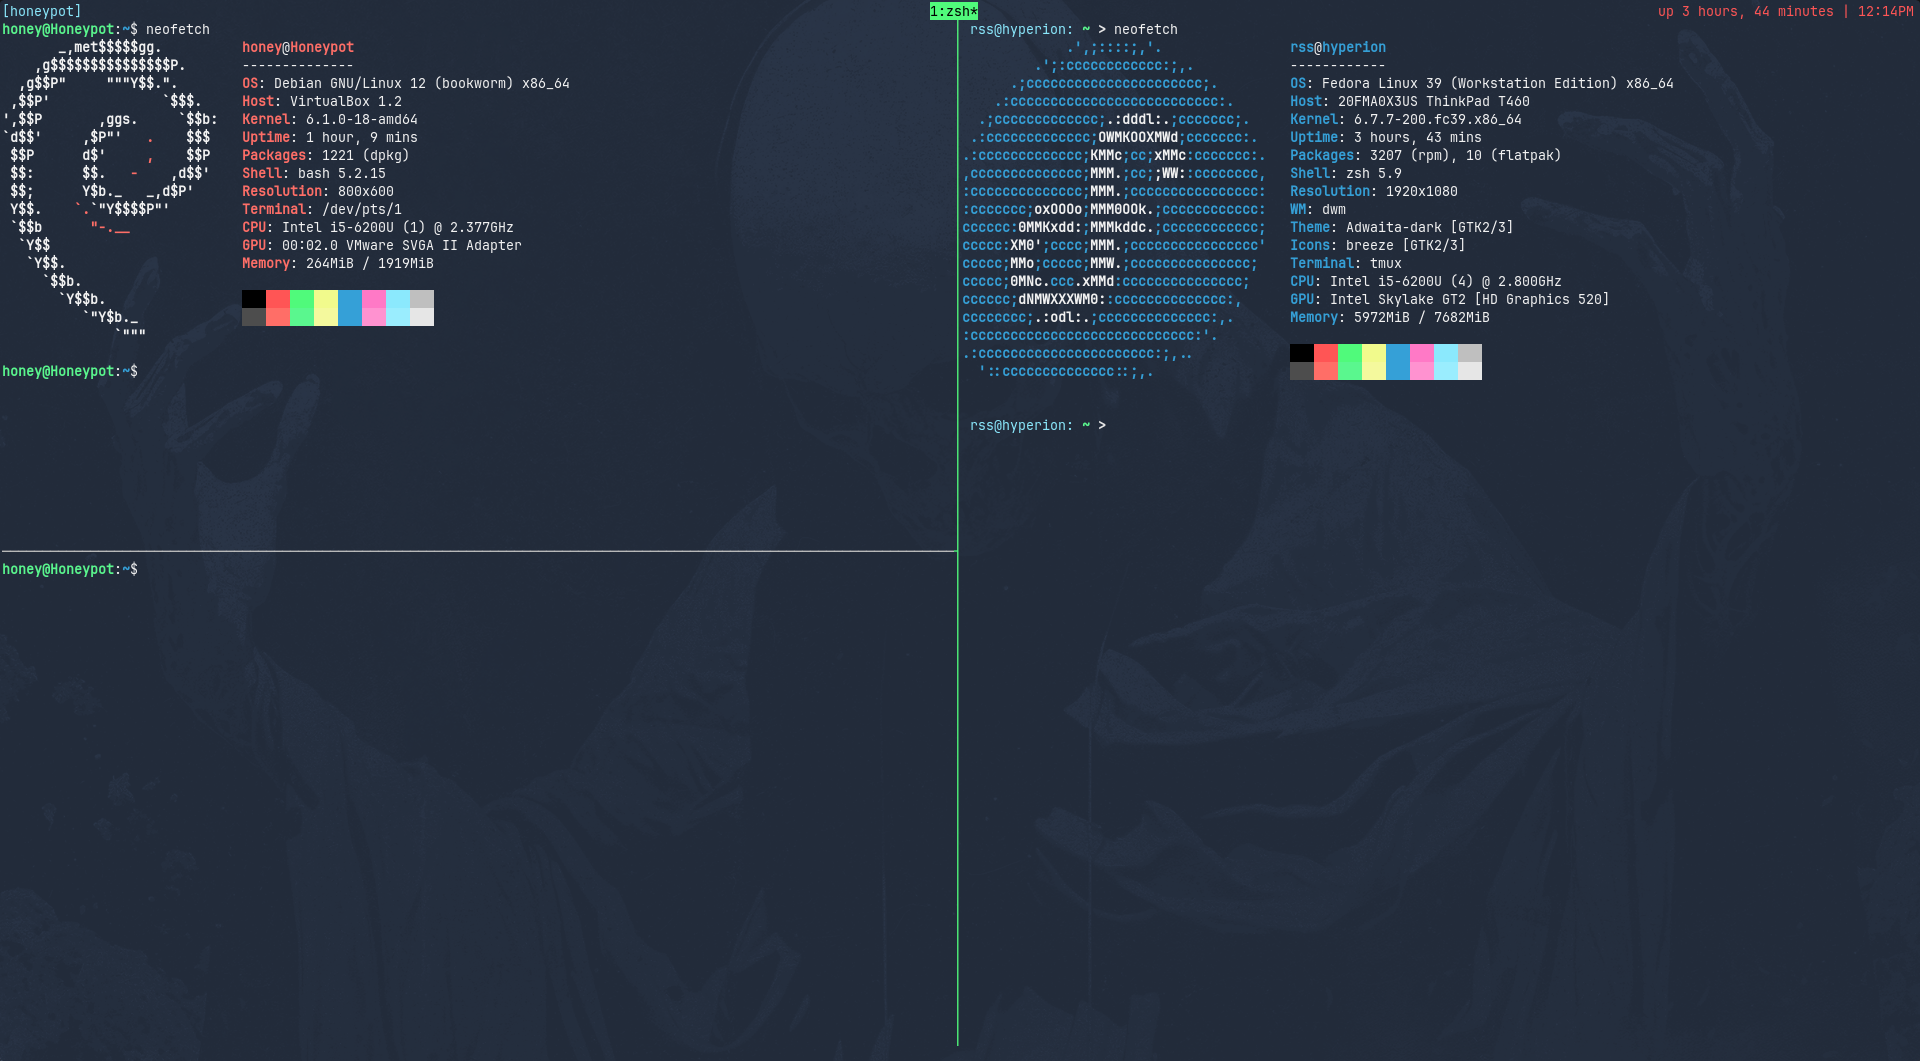
\includegraphics[scale=0.2]{SSHIMG}
  \end{center}

  Langkah pertama yang perlu dilakukan adalah untuk meng-clone repository
  Honeyport, dengan mengunakan command git sebagai berikut.

  \begin{center}
    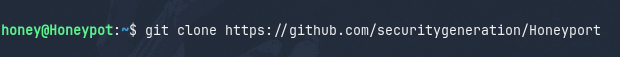
\includegraphics[scale=0.5]{GITCLONE}
  \end{center}

  Setelah repository ter-download, langkah selanjutnya adalah untuk masuk
  ke directory repository tersebut.

  \begin{center}
    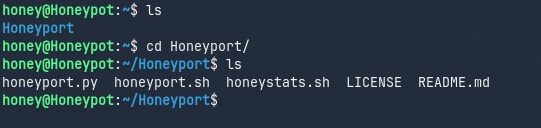
\includegraphics[scale=0.5]{HONEYPORTDIR}
  \end{center}

  Lalu, untuk meng-inisialisasi port listener, kita perlu menjalankan
  script "honeyport.sh" seperti berikut.

  \begin{center}
    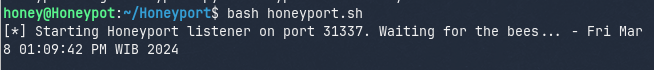
\includegraphics[scale=0.5]{HONEYPORTEXEC}
  \end{center}

  Bisa dilihat listener nya sudah terinisialisasi, dan secara default akan
  mendengarkan 31337.

  Setting untuk port apa yang harus didengarkan dapat diatur dengan meng-edit
  bash script tersebut, setting untuk script terdapat di awal script seperti
  berikut.

  \begin{center}
    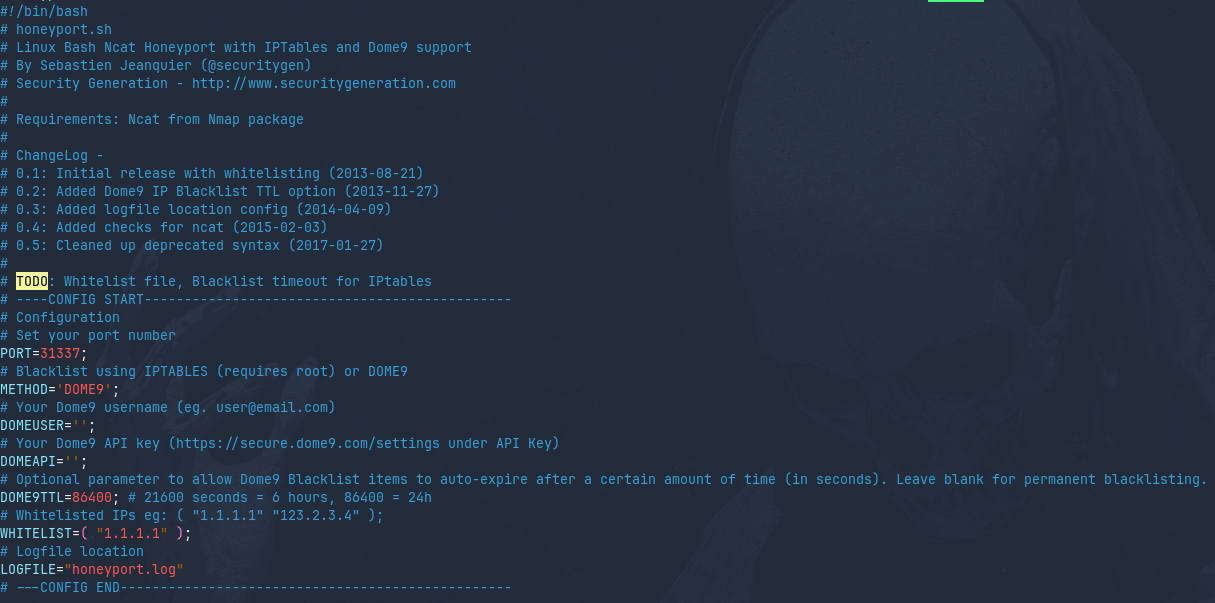
\includegraphics[scale=0.3]{HONEYPORTCONF}
  \end{center}

  Dan untuk setting yang menentukan port apa yang dipakai ada di variable
  PORT.

  \begin{center}
    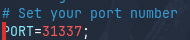
\includegraphics[scale=0.8]{PORTCONF}
  \end{center}

  Setelah proses listener berjalan, kita sekarang bisa mencoba untuk menyambung
  ke port tersebut.

  Untuk menyambung ke port tersebut dapat menggunakan tool atau command seperti
  nc, ssh, atau hal yang serupa, script Honeyport sendiri tidak akan memilah
  permintaan koneksi yang akan di didengar, maka command apapun yang biasanya
  digunakan untuk menyambung kesuatu sistem entah itu remote atau tidak akan
  dianggap oleh script sama saja.

  Command yang saya gunakan adalah ncat, ncat bisa digunakan hampir sama dengan
  ssh namun memiliki lebih banyak fitur, seperti redireksi port, proxy, authentikasi,
  dan lebih banyak lagi, bahkan ketika red-teaming ncat atau netcat biasa digunakan
  untuk mendapatkan reverse-shell.

  Perintah ncat yang digunakan adalah sebagai berikut.

  \begin{center}
    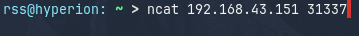
\includegraphics[scale=0.8]{NCATCMD}
  \end{center}

  Dan ketika kita melihat proses listener akan terlihat ada percobaan koneksi.

  \begin{center}
    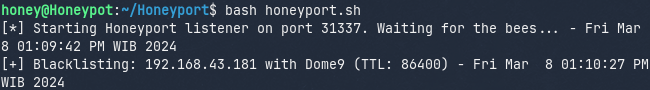
\includegraphics[scale=0.5]{NCATRESP}
  \end{center}

  Hal yang serupa akan juga terjadi kita kita menggunakan perintah ssh.

  \begin{center}
    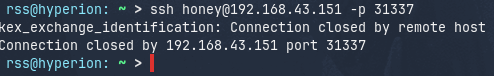
\includegraphics[scale=0.8]{SSHCMD}
  \end{center}

  Dan sama seperti sebelumnya, listener akan menampilkan hal yang sama.

  \begin{center}
    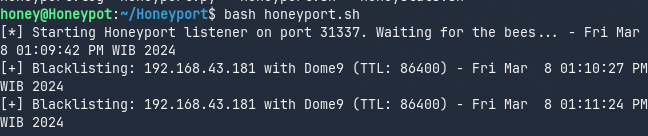
\includegraphics[scale=0.5]{SSHRESP}
  \end{center}

  Data updaya koneksi juga terdapat di logfile, yang akan diupdate tiap ada
  upaya koneksi, logfile ini hanya berisikan ip dan port apa yang ia coba sambung,
  logfile dapat ditampilkan menggunakan bash script lain yang disediakan di
  repository.

  \begin{center}
    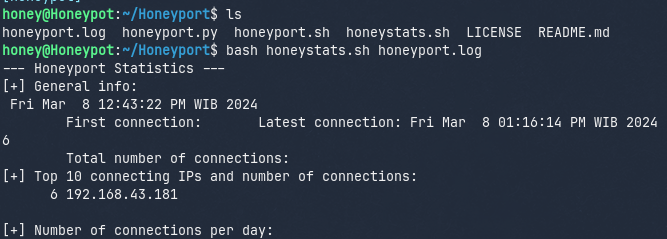
\includegraphics[scale=0.5]{LOGOUTPUT}
  \end{center}

  Dari demonstrasi diatas dapat dilihat kinerja dasar suatu honeypot, yaitu sebagai
  information-gatherer dari sebuah attacker, dan meski informasi yang didapat mungkin
  hanya ip nya, jika dikombinasikan dengan firewall atau IDS, sistem yang memanfaatkan
  lapisan honeypot di dalam sistem keamanannya akan jauh lebih efektif karena
  dapat mencegah percobaaan lebih lanjut dari si penyerang dengan cepat mem-blacklist
  atau meblokir ip tersebut.

\end{document}
